\chapter{Scenarios Overview}
\label{ch:scenarios}
% ##################################################################################################################

\hfill \textbf{Authors:} Andreas Horni, Marcel Rieser, Kai Nagel

\begin{center} 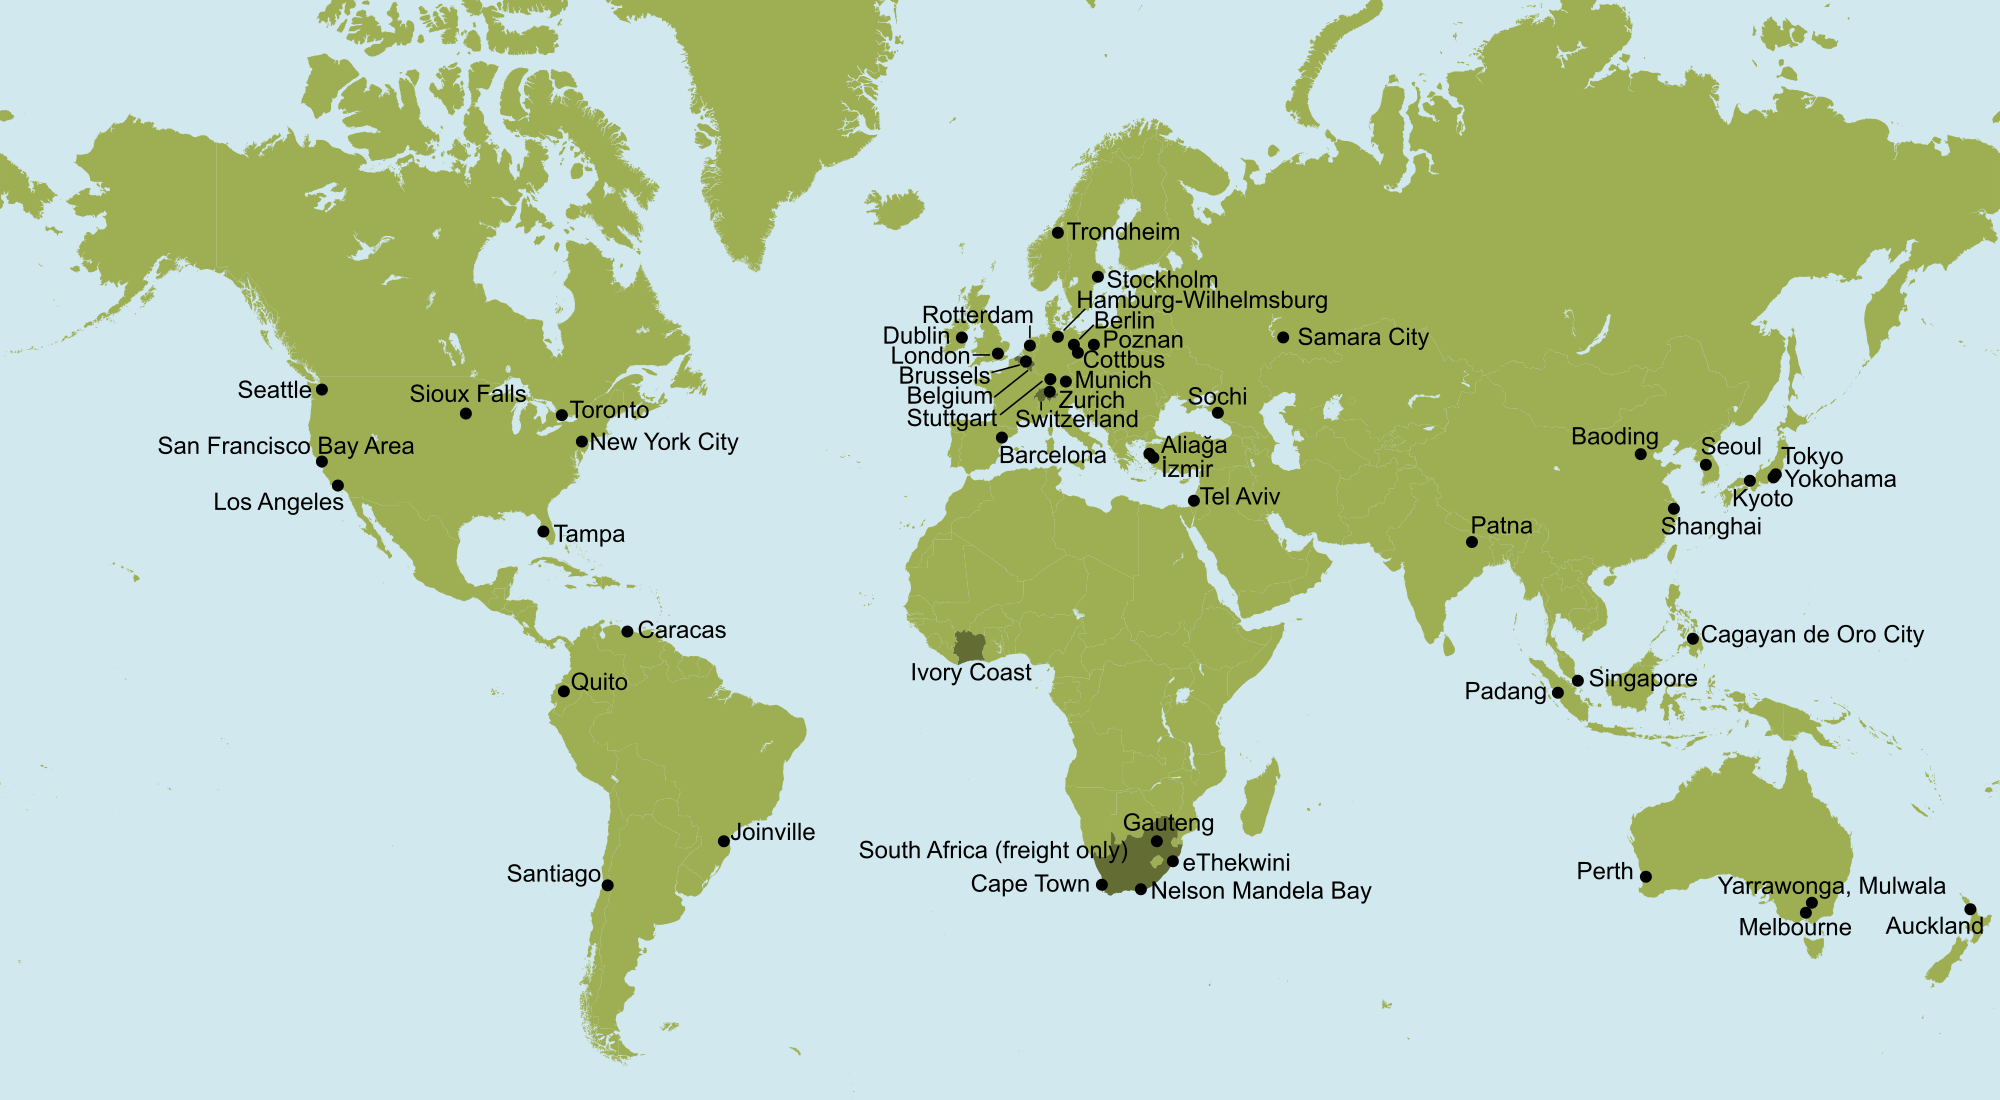
\includegraphics[width=0.7\textwidth, angle=0]{./scenarios/figures/MATSimModelsMap} \end{center}

% ##################################################################################################################
This last book part summarizes \gls{matsim} scenarios as located on the map in Figure~\ref{fig:scenarios} and listed at \citet[][]{MATSIM-Scenarios_Webpage_2015}).

Many scenarios are not public due to data privacy issues. However, knowing about the general methods and approaches adopted for scenario creation and hearing about problems faced thereby might significantly support the building of new scenarios. Content basically covers information on study area, population and demand generation, activity locations, network, simulated modes, calibration and validation, achieved results, associated projects, where to find more, where emphasis is put on specialties of a certain scenario, be it parsimonious data usage procedures, special modules used, or special modes simulated (such as the parataxis in the Gauteng scenario). Some of the scenarios are used since years with a continuous further development. We target at reporting, the latest version. 

Different levels of \gls{matsim} involvement are possible. For some regions and projects, \gls{matsim} is, for example, only used for traffic assignment, whereas for others the complete demand is endogenously handled. Couplings with other forecasting models for transport demand generation have been successfully applied such as the coupling with \gls{tasha} for Toronto or the combination of \gls{matsim} with the activity-based transport model of Tel Aviv.

\createfigure%
{Scenarios overview}%
{Scenarios overview}%
{\label{fig:scenarios}}%
{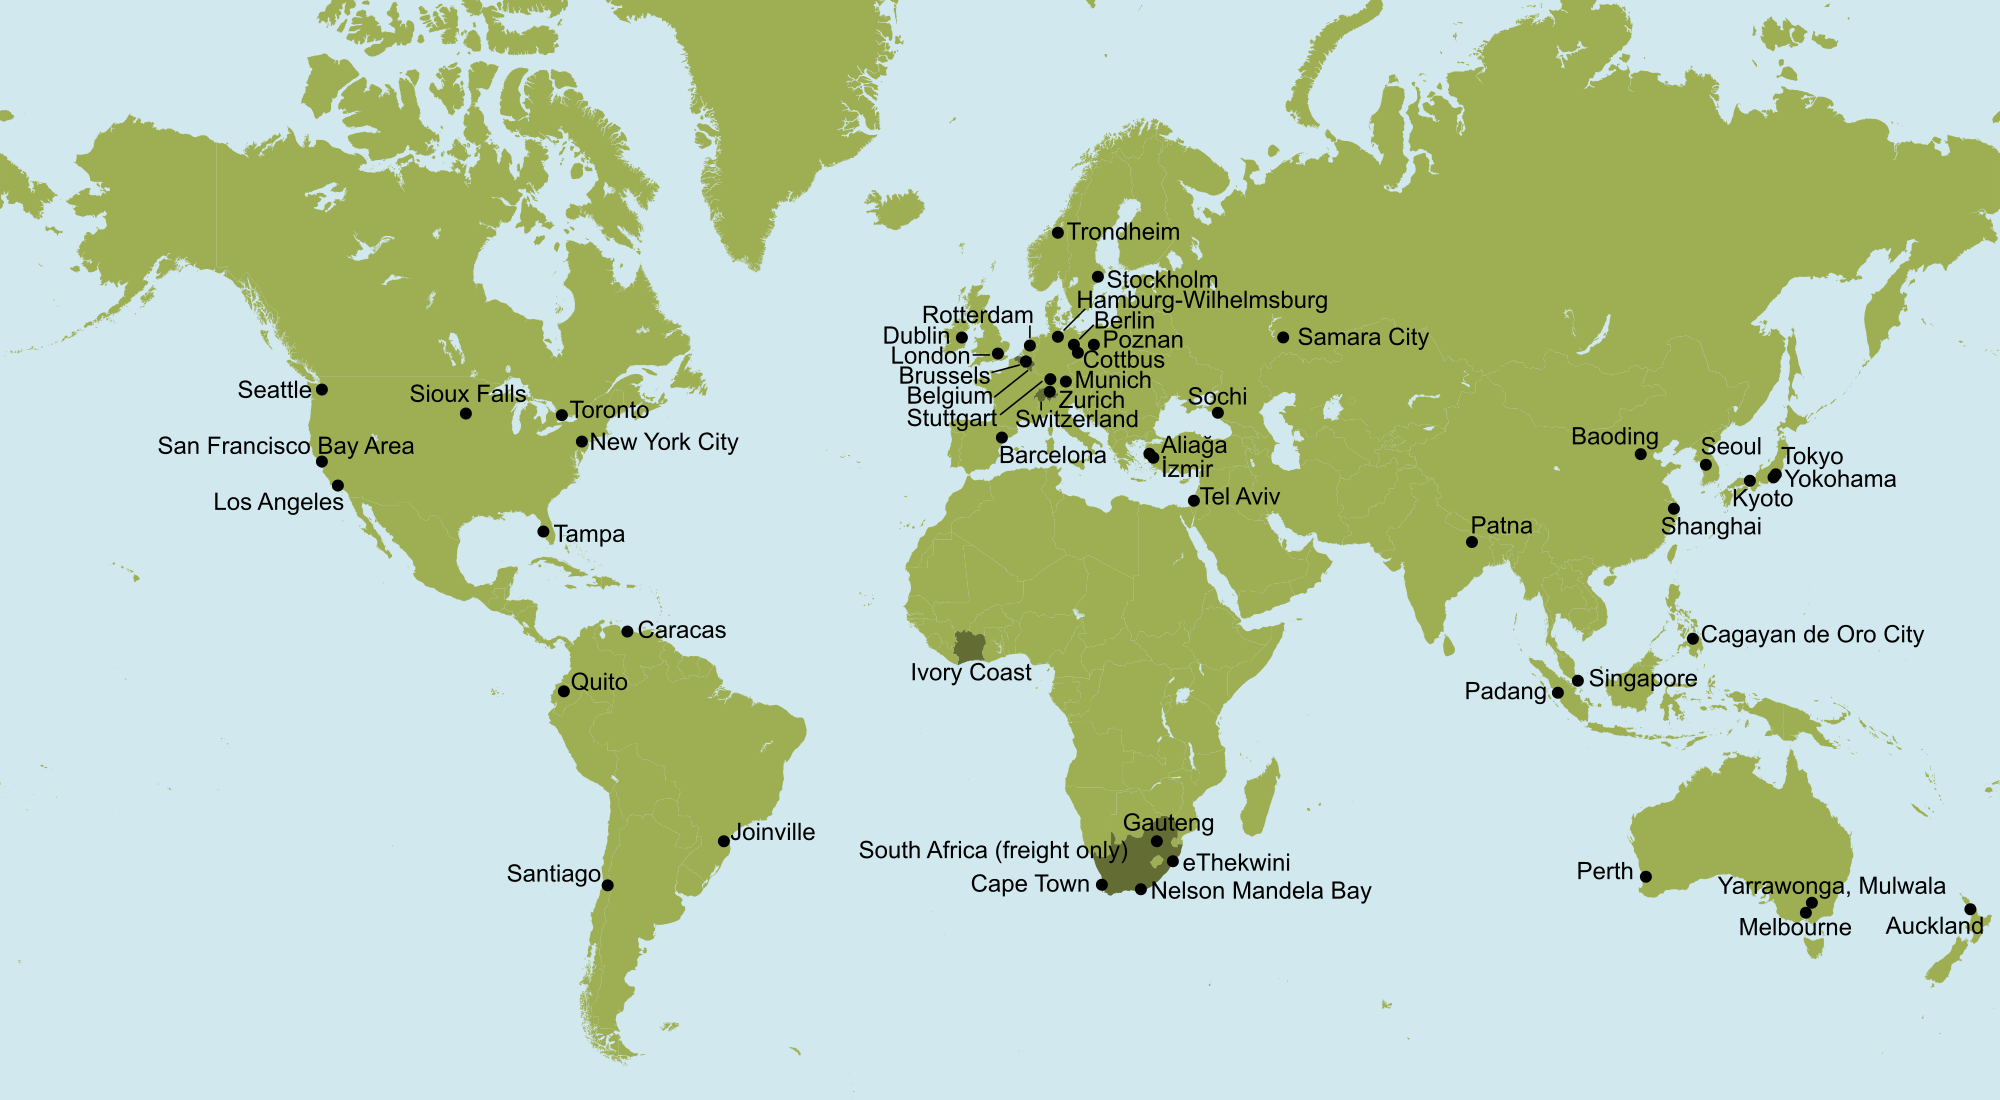
\includegraphics[width=0.99\textwidth, angle=0]{./scenarios/figures/MATSimModelsMap}}%
{}

% ==================================================================================================================
%Further models are available or currently being developed \citep[][]{Axhausen_unpub_Hong_Kong_2013, MATSIM-T-Scenarios_Webpage_2014}: 
% Izmir, 'yalcin.alver@ege.edu.tr'; 'mmetinm@gmail.com' 
% Aliaga, 'pelin.onelcin@ege.edu.tr'
% Boading (China), Chengxiang Zhuge, Chunfu Shao, Jian Gao, Meng Meng and Weiyang Xu: 'gaojian615@126.com'; 'zgcx615@126.com'; 'xutryever@126.com'; 'cfshao@bjtu.edu.cn'; 'weiyangxu23@126.com'
% Ivory Coast (Zilske), 
% LA (Balmer, unfinished), 
% Kyoto (who?)
% Santiago (who?)
% all contacted, where author known.

% ##################################################################################################################
%\section{Discussion and TODOs}
%Will be commented, when chapter is finished. Make final results traceable.

%\ah{
%- region description (characteristics, stats, ...)
%- population (popgen, Balmi plug together)
%- facilities
%- network
%- utility function (estimated, how derived)
%- pt (simulated, pseudo pt)
%- modes
%- freight (siehe keynotes Kai)
%- border crossers/boundary effects
%
%data sources
%methods applied
%
%- special problems faced \& solutions found
%
%- simulation quality
%- calibration \& validation (+available data)
%
%- purpose and sponsor/client
%- associated projects -> see Section \ref{sec:projects}
%
%- specialties: parataxis in Gauteng, connections to other sims (Toronto, Tel-Aviv)
%}

% ##################################################################################################################
